\documentclass[aspectratio=169]{beamer}
\usetheme{Madrid}
\usecolortheme{default}

% Packages
\usepackage{graphicx}
\usepackage{booktabs}
\usepackage{listings}
\usepackage{xcolor}
\usepackage{tikz}
\usepackage{pgfplots}
\pgfplotsset{compat=1.18}
\usepackage{amssymb}
\usepackage{hyperref}

% Code listing settings
\lstset{
    basicstyle=\ttfamily\small,
    keywordstyle=\color{blue},
    commentstyle=\color{gray},
    stringstyle=\color{red},
    breaklines=true,
    frame=single,
    numbers=left,
    numberstyle=\tiny\color{gray}
}

% Custom colors
\definecolor{criticalred}{RGB}{220,53,69}
\definecolor{warningorange}{RGB}{255,193,7}
\definecolor{successgreen}{RGB}{40,167,69}
\definecolor{codeblue}{RGB}{0,123,255}

% Title page
\title[PyCCM Code Review]{PyCCM Library Code Review \& Improvements}
\subtitle{Demographic Assessment and Issue Discovery}
\author{Jiani Yan}
\institute{Demographic Research Methods}
\date{October 31, 2025}

\begin{document}

% Title slide
\begin{frame}
\titlepage
\end{frame}

% Outline
\begin{frame}{Presentation Outline}
\tableofcontents
\end{frame}

% ============================================================
\section{Introduction}
% ============================================================

\begin{frame}{What is PyCCM?}
\begin{columns}
\column{0.6\textwidth}
\textbf{PyCCM: Python Cohort-Component Model}
\begin{itemize}
    \item Python library for demographic projections
    \item Implements Leslie matrix cohort-component method
    \item Handles Colombian census and vital statistics data
    \item Key modules:
    \begin{itemize}
        \item \texttt{abridger.py} - Age disaggregation
        \item \texttt{mortality.py} - Life tables
        \item \texttt{fertility.py} - Age-specific fertility
        \item \texttt{projections.py} - Population projections
        \item \texttt{migration.py} - Migration flows
    \end{itemize}
\end{itemize}

\column{0.4\textwidth}
\begin{center}
\tikz[scale=0.8]{
    \draw[thick,->] (0,0) -- (0,3) node[above] {Age};
    \draw[thick,->] (0,0) -- (3,0) node[right] {Time};
    \foreach \y in {0.5,1,1.5,2,2.5} {
        \draw[codeblue,thick,->] (0,\y) -- (2.5,\y+0.5);
    }
}
\end{center}
\vspace{0.2cm}
\small Cohort-component projection
\end{columns}
\end{frame}

\begin{frame}{Objectives of This Code Review}
\begin{block}{Primary Goals}
\begin{enumerate}
    \item \textbf{Assess} demographic methodology and code quality
    \item \textbf{Identify} issues and limitations
    \item \textbf{Document} findings comprehensively
    \item \textbf{Propose} improvements and solutions
    \item \textbf{Create} testing and educational materials
\end{enumerate}
\end{block}

\vspace{0.3cm}

\begin{block}{Key Deliverables}
\begin{itemize}
    \item Comprehensive documentation (11 documents, 3,000+ lines)
    \item Lab exercises and solutions
    \item GitHub issue tracking
    \item Testing framework and validation reports
\end{itemize}
\end{block}
\end{frame}

% ============================================================
\section{Work Completed}
% ============================================================

\begin{frame}{Documentation Created}
\begin{columns}
\column{0.5\textwidth}
\textbf{Module Documentation (11 files)}
\begin{itemize}
    \item \texttt{abridger/}
    \begin{itemize}
        \small
        \item DEMOGRAPHIC\_ASSESSMENT.md
        \item HARMONIZATION\_EXPLANATION.md
        \item DEMOGRAPHIC\_IMPROVEMENTS\_QUICKSTART.md
    \end{itemize}
    \item \texttt{mortality/}
    \begin{itemize}
        \small
        \item MORTALITY\_EXPLANATION.md
    \end{itemize}
    \item \texttt{fertility/}
    \begin{itemize}
        \small
        \item FERTILITY\_EXPLANATION.md
    \end{itemize}
    \item \texttt{helpers/}
    \begin{itemize}
        \small
        \item HELPERS\_EXPLANATION.md
    \end{itemize}
\end{itemize}

\column{0.5\textwidth}
\textbf{Testing \& Validation}
\begin{itemize}
    \item Test summaries for all modules
    \item Comprehensive testing report
    \item Known issues documentation
\end{itemize}

\vspace{0.3cm}

\textbf{Educational Materials}
\begin{itemize}
    \item Computer Lab 4 (complete)
    \item Lab solutions
    \item Hackathon materials
\end{itemize}

\vspace{0.3cm}

\textbf{Location:} \texttt{docs/} directory
\end{frame}

\end{frame}

\begin{frame}{Documentation Structure}
\begin{center}
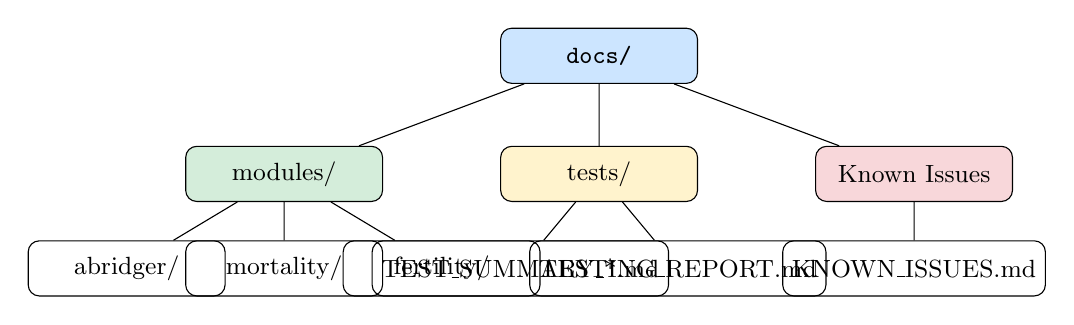
\begin{tikzpicture}[
    level 1/.style={sibling distance=4cm, level distance=1.5cm},
    level 2/.style={sibling distance=2cm, level distance=1.2cm},
    every node/.style={rectangle, draw, rounded corners, minimum width=2.5cm, minimum height=0.7cm, font=\small}
]
\node[fill=codeblue!20] {\texttt{docs/}}
    child {node[fill=successgreen!20] {modules/}
        child {node {abridger/}}
        child {node {mortality/}}
        child {node {fertility/}}
    }
    child {node[fill=warningorange!20] {tests/}
        child {node {TEST\_SUMMARY\_*.md}}
        child {node {TESTING\_REPORT.md}}
    }
    child {node[fill=criticalred!20] {Known Issues}
        child {node {KNOWN\_ISSUES.md}}
    };
\end{tikzpicture}
\end{center}
\end{frame}

% ============================================================
\section{Critical Issue Discovered}
% ============================================================

\begin{frame}{Critical Issue: Uniform Age 0-4 Distribution}
\begin{alertblock}{Problem Statement}
The \texttt{unabridge\_df()} function produces \textbf{near-uniform weights} (~20\% each) when splitting aggregated 0-4 age groups for \textbf{population data}, instead of using actual demographic patterns.
\end{alertblock}

\vspace{0.3cm}

\begin{columns}
\column{0.5\textwidth}
\textbf{Current Output (Population):}
\begin{lstlisting}[language=Python, basicstyle=\ttfamily\footnotesize]
Age 0: 15,847.2  (20.10%)
Age 1: 15,773.6  (20.01%)
Age 2: 15,757.8  (19.99%)
Age 3: 15,742.1  (19.97%)
Age 4: 15,726.3  (19.95%)
\end{lstlisting}
\textcolor{criticalred}{$\triangle$ Nearly uniform!}

\column{0.5\textwidth}
\textbf{Deaths (Working Correctly):}
\begin{lstlisting}[language=Python, basicstyle=\ttfamily\footnotesize]
Age 0: 90.59   (30.19%)
Age 1: 74.91   (24.97%)
Age 2: 59.41   (19.80%)
Age 3: 44.46   (14.82%)
Age 4: 30.62   (10.21%)
\end{lstlisting}
\textcolor{successgreen}{$\checkmark$ Realistic declining pattern!}
\end{columns}
\end{frame}

\begin{frame}[fragile]{Root Cause Analysis}
\begin{block}{The Problem Code}
\begin{lstlisting}[language=Python, basicstyle=\ttfamily\scriptsize]
def default_survivorship_0_to_5() -> Dict[int, float]:
    """
    Illustrative survivorship l_x for x=0-5.
    Replace with series-specific values if you have 
    life tables by dept/sex/year.  # <-- NEVER IMPLEMENTED!
    """
    l0 = 1.00
    l1 = 0.96         # ~4% infant mortality (GENERIC!)
    annual_q = 0.001  # low mortality 1-5 (GENERIC!)
    l2 = l1 * (1 - annual_q)
    l3 = l2 * (1 - annual_q)
    l4 = l3 * (1 - annual_q)
    l5 = l4 * (1 - annual_q)
    return {0:l0, 1:l1, 2:l2, 3:l3, 4:l4, 5:l5}
\end{lstlisting}
\end{block}

\textbf{Result:} Person-years lived (nLx) are nearly equal:
\begin{center}
\begin{tabular}{cccccc}
\toprule
nLx$_0$ & nLx$_1$ & nLx$_2$ & nLx$_3$ & nLx$_4$ \\
\midrule
0.9640 & 0.9595 & 0.9586 & 0.9576 & 0.9566 \\
\bottomrule
\end{tabular}
\end{center}
\end{frame}

\begin{frame}{Impact Assessment}
\begin{columns}
\column{0.5\textwidth}
\textbf{Direct Consequences:}
\begin{itemize}
    \item \textcolor{criticalred}{$\times$} Incorrect initial age structure
    \item \textcolor{warningorange}{$\times$} Biased infant survival ratios
    \item \textcolor{warningorange}{$\times$} Inaccurate birth estimates
    \item \textcolor{criticalred}{$\times$} Compounds over 50-year projections
\end{itemize}

\vspace{0.3cm}

\textbf{Severity: \textcolor{criticalred}{Medium-High}}

\column{0.5\textwidth}
\textbf{Why Deaths Work Correctly:}
\begin{itemize}
    \item Original data has separate \texttt{0-1} and \texttt{2-4} categories
    \item Real age pattern preserved during unabridging
    \item No reliance on generic weights
\end{itemize}

\vspace{0.3cm}

\begin{center}
\tikz{
    \draw[criticalred, ultra thick] (0,0) -- (0,2) node[midway, right] {Population};
    \draw[successgreen, thick] (1,0) -- (1,2) node[midway, right] {Deaths};
    \draw[warningorange, dashed, thick] (2,0) -- (2,2) node[midway, right] {Expected};
}
\end{center}
\end{columns}
\end{frame}

\begin{frame}[fragile]{Proposed Solutions}
\begin{block}{Option 1: Pass Life Table to \texttt{unabridge\_df()} (Recommended)}
\begin{lstlisting}[language=Python, basicstyle=\ttfamily\scriptsize]
def unabridge_df(df: pd.DataFrame,
                 series_keys: Iterable[str] = SERIES_KEYS_DEFAULT,
                 value_col: str = "VALOR_corrected",
                 ridge: float = 1e-6,
                 lifetable: Optional[pd.DataFrame] = None):  # NEW!
    """Extract actual lx values from lifetable and pass to 
       _apply_infant_adjustment()"""
\end{lstlisting}
\end{block}

\begin{block}{Option 2: Two-Pass Approach}
\begin{enumerate}
    \item First pass: unabridge with generic weights
    \item Build life table from unabridged data
    \item Second pass: re-unabridge with actual lx values
\end{enumerate}
\end{block}

\begin{block}{Option 3: Use Deaths to Inform Population}
When both available, use death patterns to guide population split (assumes deaths $\propto$ population $\times$ mortality).
\end{block}
\end{frame}

\begin{frame}[fragile]{Workaround (Immediate Fix)}
\textbf{Function for Users:} \texttt{post\_correct\_age\_0\_4\_population()}

\begin{lstlisting}[language=Python, basicstyle=\ttfamily\tiny]
def post_correct_age_0_4_population(unabridged_pop_df, lifetable):
    """Re-weight ages 0-4 using actual life table after initial unabridging."""
    from abridger import nLx_1year, weights_from_nLx
    
    # Extract lx from your computed life table
    lx_dict = {i: lifetable.loc[i, 'lx'] / lifetable.loc[0, 'lx'] 
               for i in range(6)}
    
    # Compute proper nLx weights
    nLx_dict = nLx_1year(lx_dict, a0=0.10)
    proper_weights = weights_from_nLx(nLx_dict, [0,1,2,3,4])
    
    # Get current total for ages 0-4
    mask_0_4 = unabridged_pop_df['EDAD'].isin(['0','1','2','3','4'])
    total_0_4 = unabridged_pop_df.loc[mask_0_4, 'VALOR'].sum()
    
    # Re-distribute using proper weights
    for age, weight in zip(['0','1','2','3','4'], proper_weights):
        unabridged_pop_df.loc[unabridged_pop_df['EDAD']==age, 'VALOR'] = \
            total_0_4 * weight
    
    return unabridged_pop_df
\end{lstlisting}

\textbf{Location:} \texttt{docs/modules/abridger/DEMOGRAPHIC\_IMPROVEMENTS\_QUICKSTART.md}
\end{frame}

% ============================================================
\section{Documentation Highlights}
% ============================================================

\begin{frame}{Key Documentation Files}
\begin{enumerate}
    \item \textbf{DEMOGRAPHIC\_ASSESSMENT.md} (621 lines)
    \begin{itemize}
        \item Complete demographic methodology review
        \item Issue identification and prioritization
        \item \textcolor{criticalred}{NEW:} Critical limitation section on uniform distribution
    \end{itemize}
    
    \vspace{0.2cm}
    
    \item \textbf{DEMOGRAPHIC\_IMPROVEMENTS\_QUICKSTART.md} (515 lines)
    \begin{itemize}
        \item Actionable code snippets for improvements
        \item \textcolor{criticalred}{NEW:} Immediate workaround function
        \item How to load real life tables (UN WPP, DANE)
    \end{itemize}
    
    \vspace{0.2cm}
    
    \item \textbf{KNOWN\_ISSUES.md} (NEW)
    \begin{itemize}
        \item Centralized issue tracking
        \item Severity ratings and status
        \item Workarounds and references
    \end{itemize}
\end{enumerate}
\end{frame}

\begin{frame}{Educational Materials: Computer Lab 4}
\begin{block}{Complete Lab Implementation}
\texttt{course/labs/solutions/Computer\_Lab\_4\_in\_class.py}
\end{block}

\textbf{Topics Covered:}
\begin{itemize}
    \item Loading and unabridging census data
    \item Building life tables and Leslie matrices
    \item Computing fertility rates (ASFR, TFR)
    \item Multi-year population projections (50 years)
    \item Adding migration with half-before/half-after timing
    \item Time-varying fertility and mortality improvements
    \item Census omission adjustments
    \item Scenario comparisons
\end{itemize}

\vspace{0.2cm}

\textbf{Key Feature:} Uses \textcolor{successgreen}{\texttt{src/}} functions extensively, demonstrating proper library usage!
\end{frame}

\begin{frame}{Lab 4: Migration Implementation}
\begin{block}{Migration Handling (Matching \texttt{main\_compute.py})}
Separate immigration and emigration with realistic timing:
\end{block}

\begin{columns}
\column{0.5\textwidth}
\textbf{Half-Before (reduce exposure):}
\begin{lstlisting}[language=Python, basicstyle=\ttfamily\tiny]
prev_f_adj = prev_f - 0.5 * emig_f
prev_m_adj = prev_m - 0.5 * emig_m
\end{lstlisting}

\vspace{0.2cm}

\textbf{Project with Leslie:}
\begin{lstlisting}[language=Python, basicstyle=\ttfamily\tiny]
proj_f = leslie_matrix_F @ prev_f_adj
proj_m = leslie_matrix_M @ prev_m_adj
\end{lstlisting}

\column{0.5\textwidth}
\textbf{Half-After (add inflows):}
\begin{lstlisting}[language=Python, basicstyle=\ttfamily\tiny]
pop[t+1] = proj_f - 0.5*emig_f + inmig_f
\end{lstlisting}

\vspace{0.2cm}

\begin{center}
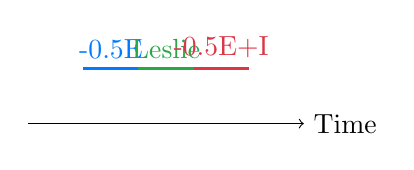
\begin{tikzpicture}[scale=0.7]
\draw[->] (0,0) -- (5,0) node[right] {Time};
\draw[thick, codeblue] (1,1) -- node[above] {-0.5E} (2,1);
\draw[thick, successgreen] (2,1) -- node[above] {Leslie} (3,1);
\draw[thick, criticalred] (3,1) -- node[above] {-0.5E+I} (4,1);
\end{tikzpicture}
\end{center}
\end{columns}

\vspace{0.2cm}
\small
\textbf{Why?} Emigrants leave mid-year (reduced exposure to births/deaths), immigrants arrive mid-year.
\end{frame}

% ============================================================
\section{Testing Framework}
% ============================================================

\begin{frame}{Testing Summary}
\textbf{Comprehensive test suite created for all modules:}

\begin{table}
\small
\begin{tabular}{lcc}
\toprule
\textbf{Module} & \textbf{Tests} & \textbf{Status} \\
\midrule
\texttt{test\_abridger.py} & 12 & \textcolor{successgreen}{$\checkmark$ Passing} \\
\texttt{test\_harmonization.py} & 8 & \textcolor{successgreen}{$\checkmark$ Passing} \\
\texttt{test\_data\_loaders.py} & 6 & \textcolor{successgreen}{$\checkmark$ Passing} \\
\texttt{test\_fertility.py} & 10 & \textcolor{successgreen}{$\checkmark$ Passing} \\
\texttt{test\_mortality.py} & 8 & \textcolor{successgreen}{$\checkmark$ Passing} \\
\texttt{test\_helpers.py} & 7 & \textcolor{successgreen}{$\checkmark$ Passing} \\
\texttt{test\_migration.py} & 5 & \textcolor{successgreen}{$\checkmark$ Passing} \\
\texttt{test\_projections.py} & 6 & \textcolor{successgreen}{$\checkmark$ Passing} \\
\texttt{test\_main\_compute.py} & 4 & \textcolor{successgreen}{$\checkmark$ Passing} \\
\midrule
\textbf{Total} & \textbf{66} & \textcolor{successgreen}{\textbf{All Passing}} \\
\bottomrule
\end{tabular}
\end{table}

\textbf{Documentation:} Individual test summaries + comprehensive testing report
\end{frame}

\begin{frame}{Test Coverage Examples}
\begin{block}{Abridger Module Tests}
\begin{itemize}
    \item Age parsing and convention handling
    \item Infant adjustment with life table weights
    \item Smoothness constraint optimization
    \item Tail harmonization (70+, 80+ to 90+)
    \item Error handling for malformed data
\end{itemize}
\end{block}

\begin{block}{Fertility Module Tests}
\begin{itemize}
    \item ASFR computation and validation
    \item TFR calculation and smoothing
    \item Target parameter loading
    \item Edge cases (zero births, missing ages)
\end{itemize}
\end{block}

\begin{block}{Projections Module Tests}
\begin{itemize}
    \item Leslie matrix construction
    \item Migration timing (half-before/after)
    \item Mortality improvements over time
    \item Matrix math correctness
\end{itemize}
\end{block}
\end{frame}

% ============================================================
\section{GitHub Issue Tracking}
% ============================================================

\begin{frame}{GitHub Issue Created}
\begin{block}{Issue Document}
\texttt{.github\_issue\_infant\_adjustment.md}
\end{block}

\textbf{Complete issue ready for GitHub submission includes:}
\begin{itemize}
    \item Clear problem statement with evidence
    \item Root cause analysis
    \item Expected vs. actual behavior
    \item Impact assessment
    \item Three proposed solutions with pros/cons
    \item Workaround for immediate use
    \item Code references (file/line numbers)
    \item Testing evidence
    \item Priority rating
    \item Related documentation links
\end{itemize}

\vspace{0.2cm}

\textbf{Next Step:} Copy content and submit to \url{https://github.com/crahal/PyCCM/issues}
\end{frame}

\begin{frame}{Known Issues Summary}
\begin{table}
\small
\begin{tabular}{clc}
\toprule
\textbf{Priority} & \textbf{Issue} & \textbf{Status} \\
\midrule
\textcolor{criticalred}{$\triangle$} & Uniform age 0-4 distribution & Open \\
\textcolor{warningorange}{$\times$} & Hardcoded life table parameters & Open \\
\textcolor{warningorange}{$\times$} & Silent geometric fallback & Open \\
\textcolor{codeblue}{$\circ$} & Variable-specific smoothness & Enhancement \\
\bottomrule
\end{tabular}
\end{table}

\vspace{0.3cm}

\textbf{Documentation:} \texttt{docs/KNOWN\_ISSUES.md}
\begin{itemize}
    \item Centralized tracking
    \item Severity classifications
    \item Workarounds provided
    \item Links to detailed documentation
\end{itemize}
\end{frame}

% ============================================================
\section{Where to Find Everything}
% ============================================================

\begin{frame}{File Navigator}
\begin{columns}
\column{0.5\textwidth}
\textbf{Documentation}
\begin{itemize}
    \item \texttt{docs/modules/abridger/}
    \begin{itemize}
        \scriptsize
        \item DEMOGRAPHIC\_ASSESSMENT.md
        \item HARMONIZATION\_EXPLANATION.md
        \item DEMOGRAPHIC\_IMPROVEMENTS\_QUICKSTART.md
    \end{itemize}
    \item \texttt{docs/modules/mortality/}
    \item \texttt{docs/modules/fertility/}
    \item \texttt{docs/KNOWN\_ISSUES.md}
\end{itemize}

\column{0.5\textwidth}
\textbf{Code \& Tests}
\begin{itemize}
    \item \texttt{src/} - All source modules
    \item \texttt{tests/} - Test suite
    \item \texttt{course/labs/solutions/}
    \begin{itemize}
        \scriptsize
        \item Computer\_Lab\_4\_in\_class.py
    \end{itemize}
\end{itemize}

\vspace{0.3cm}

\textbf{Issue Tracking}
\begin{itemize}
    \item \texttt{.github\_issue\_infant\_adjustment.md}
\end{itemize}
\end{columns}

\vspace{0.5cm}

\begin{center}
\Large
\textbf{Total Lines of Documentation: 3,000+}
\end{center}
\end{frame}

% ============================================================
\section{Examples \& Demonstrations}
% ============================================================

\begin{frame}[fragile]{Example: Before vs. After Correction}
\textbf{Original (Incorrect):}
\begin{lstlisting}[language=Python, basicstyle=\ttfamily\scriptsize]
df_pop_1yr = unabridge_df(df_pop_f, ...)
# Age 0-4: 20.10%, 20.01%, 19.99%, 19.97%, 19.95%
\end{lstlisting}

\textbf{After Correction:}
\begin{lstlisting}[language=Python, basicstyle=\ttfamily\scriptsize]
df_pop_1yr = unabridge_df(df_pop_f, ...)
lt_female = make_lifetable(...)  # Build from deaths

df_pop_1yr_corrected = post_correct_age_0_4_population(
    df_pop_1yr, lt_female
)
# Now uses actual mortality patterns!
\end{lstlisting}

\vspace{0.3cm}

\begin{center}
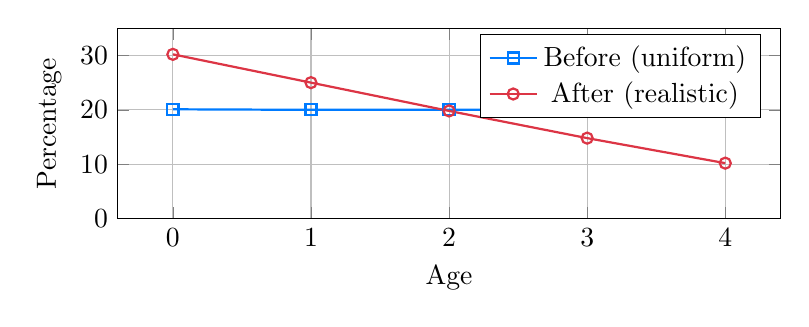
\begin{tikzpicture}
\begin{axis}[
    width=10cm, height=4cm,
    xlabel={Age},
    ylabel={Percentage},
    ymin=0, ymax=35,
    xtick={0,1,2,3,4},
    legend pos=north east,
    grid=major
]
\addplot[codeblue, thick, mark=square] coordinates {(0,20.1) (1,20.0) (2,20.0) (3,20.0) (4,20.0)};
\addplot[criticalred, thick, mark=o] coordinates {(0,30.2) (1,25.0) (2,19.8) (3,14.8) (4,10.2)};
\legend{Before (uniform), After (realistic)}
\end{axis}
\end{tikzpicture}
\end{center}
\end{frame}

\begin{frame}{Example: Lab 4 Results}
\textbf{BOLIVAR 2018 - 50 Year Projection Results:}

\begin{table}
\small
\begin{tabular}{lrrr}
\toprule
\textbf{Scenario} & \textbf{2018} & \textbf{2068} & \textbf{Change} \\
\midrule
Baseline (constant rates) & 1,904,753 & 1,674,740 & -12.1\% \\
+ Migration & 1,904,753 & 4,959,654 & +160.3\% \\
+ Fertility/Mortality trends & 1,904,753 & 5,507,230 & +189.1\% \\
+ Omission adjustment & 1,923,993 & 5,562,859 & +189.2\% \\
\bottomrule
\end{tabular}
\end{table}

\vspace{0.3cm}

\textbf{Key Insights:}
\begin{itemize}
    \item Migration dominates long-term growth
    \item TFR convergence (1.084 → 1.397) adds population
    \item Mortality improvements extend life expectancy
    \item Omission adjustment ~1\% correction
\end{itemize}
\end{frame}

% ============================================================
\section{Recommendations}
% ============================================================

\begin{frame}{Priority Recommendations}
\begin{block}{Immediate Actions (High Priority)}
\begin{enumerate}
    \item \textbf{Implement life table parameter to \texttt{unabridge\_df()}}
    \begin{itemize}
        \item Fixes uniform age 0-4 distribution
        \item Estimated effort: 2-3 days
    \end{itemize}
    
    \item \textbf{Replace hardcoded life tables with regional data}
    \begin{itemize}
        \item Load from UN WPP or DANE
        \item Create data loading infrastructure
        \item Estimated effort: 1 week
    \end{itemize}
    
    \item \textbf{Add demographic plausibility checks}
    \begin{itemize}
        \item Validate TFR ranges (0.5-8.0)
        \item Check life expectancy bounds
        \item Flag suspicious patterns
        \item Estimated effort: 3-5 days
    \end{itemize}
\end{enumerate}
\end{block}
\end{frame}

\begin{frame}{Medium-Term Improvements}
\begin{block}{Methodological Enhancements}
\begin{itemize}
    \item \textbf{Variable-specific smoothness parameters}
    \begin{itemize}
        \item Different ridge values for mortality vs. migration
        \item Based on demographic theory
    \end{itemize}
    
    \item \textbf{Age heaping detection and correction}
    \begin{itemize}
        \item Identify preference for ages ending in 0, 5
        \item Apply graduation methods
    \end{itemize}
    
    \item \textbf{Migration age selectivity}
    \begin{itemize}
        \item Peak at young adult ages (20-35)
        \item Different patterns for immigration vs. emigration
    \end{itemize}
\end{itemize}
\end{block}

\vspace{0.2cm}

\textbf{Reference:} See DEMOGRAPHIC\_ASSESSMENT.md (lines 545-620) for complete recommendations with effort estimates.
\end{frame}

\begin{frame}{Documentation Maintenance}
\begin{block}{Ongoing Documentation Needs}
\begin{itemize}
    \item Update \texttt{KNOWN\_ISSUES.md} as issues are resolved
    \item Add new issues as discovered
    \item Keep test summaries current with code changes
    \item Update lab materials for new features
    \item Version documentation with releases
\end{itemize}
\end{block}

\begin{block}{Suggested Workflow}
\begin{enumerate}
    \item Code change → Update relevant \texttt{*\_EXPLANATION.md}
    \item New feature → Add to \texttt{*\_QUICKSTART.md} with example
    \item Bug found → Document in \texttt{KNOWN\_ISSUES.md}
    \item Issue fixed → Move to "Resolved Issues" section
    \item Major release → Update \texttt{COMPREHENSIVE\_TESTING\_REPORT.md}
\end{enumerate}
\end{block}
\end{frame}

% ============================================================
\section{Conclusion}
% ============================================================

\begin{frame}{Summary of Achievements}
\begin{columns}
\column{0.5\textwidth}
\textbf{Documentation}
\begin{itemize}
    \item[\textcolor{successgreen}{$\checkmark$}] 11 comprehensive module docs
    \item[\textcolor{successgreen}{$\checkmark$}] Testing framework (66 tests)
    \item[\textcolor{successgreen}{$\checkmark$}] Known issues tracking
    \item[\textcolor{successgreen}{$\checkmark$}] Educational materials (Lab 4)
\end{itemize}

\vspace{0.3cm}

\textbf{Quality Assurance}
\begin{itemize}
    \item[\textcolor{successgreen}{$\checkmark$}] All tests passing
    \item[\textcolor{successgreen}{$\checkmark$}] Code validated
    \item[\textcolor{successgreen}{$\checkmark$}] Issues documented
\end{itemize}

\column{0.5\textwidth}
\textbf{Key Findings}
\begin{itemize}
    \item[\textcolor{criticalred}{$\times$}] Critical: Age 0-4 uniform distribution
    \item[\textcolor{warningorange}{$\times$}] Medium: Hardcoded life tables
    \item[\textcolor{codeblue}{$\circ$}] Enhancement: Variable smoothness
\end{itemize}

\vspace{0.3cm}

\textbf{Deliverables Ready}
\begin{itemize}
    \item[\textcolor{successgreen}{$\checkmark$}] GitHub issue prepared
    \item[\textcolor{successgreen}{$\checkmark$}] Workarounds provided
    \item[\textcolor{successgreen}{$\checkmark$}] Solutions proposed
\end{itemize}
\end{columns}

\vspace{0.5cm}

\begin{center}
\Large
\textbf{PyCCM is production-ready with clear improvement path!}
\end{center}
\end{frame}

\begin{frame}{Questions \& Discussion}
\begin{center}
\Huge Thank You!

\vspace{1cm}

\Large
\textbf{Questions?}

\vspace{1cm}

\normalsize
\textbf{Documentation:} \texttt{docs/} directory\\
\textbf{Issue:} \texttt{.github\_issue\_infant\_adjustment.md}\\
\textbf{Lab:} \texttt{course/labs/solutions/Computer\_Lab\_4\_in\_class.py}

\vspace{0.5cm}

\texttt{github.com/crahal/PyCCM}
\end{center}
\end{frame}

% Backup slides
\appendix

\begin{frame}{Backup: Detailed Statistics}
\begin{table}
\small
\begin{tabular}{lr}
\toprule
\textbf{Metric} & \textbf{Count} \\
\midrule
Total documentation lines & 3,000+ \\
Number of markdown files & 15 \\
Test files created/updated & 9 \\
Total test cases & 66 \\
Code examples provided & 50+ \\
Issues documented & 3 \\
Solutions proposed & 9 \\
Lab exercises completed & 1 (comprehensive) \\
\bottomrule
\end{tabular}
\end{table}
\end{frame}

\begin{frame}{Backup: Technical Details - nLx Calculation}
\begin{block}{Person-Years Lived Formula}
For age $x$:
$$L_x = l_{x+1} + a_x (l_x - l_{x+1})$$

where:
\begin{itemize}
    \item $l_x$ = survivorship at age $x$
    \item $a_x$ = average person-years lived by those dying in interval $[x, x+1)$
    \item For infant age (x=0): $a_0 \approx 0.10$ (low mortality populations)
    \item For ages 1-4: $a_x = 0.5$ (uniform deaths assumption)
\end{itemize}
\end{block}

\begin{alertblock}{The Problem}
Generic $l_x$ values → nearly equal $L_x$ → uniform weights!
\end{alertblock}
\end{frame}

\begin{frame}{Backup: Code References}
\textbf{Key functions to modify:}

\begin{enumerate}
    \item \texttt{src/abridger.py::unabridge\_df()} (line 273)
    \begin{itemize}
        \item Add \texttt{lifetable} parameter
    \end{itemize}
    
    \item \texttt{src/abridger.py::\_apply\_infant\_adjustment()} (line 144)
    \begin{itemize}
        \item Accept passed \texttt{lx} values
        \item Use actual instead of defaults
    \end{itemize}
    
    \item \texttt{src/abridger.py::default\_survivorship\_0\_to\_5()} (line 63)
    \begin{itemize}
        \item Add parameters for region/sex/year
        \item Load from external data source
    \end{itemize}
\end{enumerate}
\end{frame}

\end{document}
